% % % % % % % % % % % % % % % % % % % % % % % % % % % % % % % % % % % % % % % % % % % %
%                                                                                     %
% Short Sectioned Assignment LaTeX Template Version 1.0 (5/5/12)                      %
% This template has been downloaded from: http://www.LaTeXTemplates.com               %
%                                                                                     %
% Original author:  Frits Wenneker (http://www.howtotex.com)                          %
%                                                                                     %
% Modified by: Fco Javier Sueza Rodríguez (fcosueza@disroot.org)                      %
%                                                                                     %
% Changes:                                                                            %
%	    - Custom Chapters, Sections and Subsections (titlesec package)                %
%           - Document type scrbook (oneside)                                         %
%           - Use babel-lang-spanish package and marvosym                             %
%           - Use hyperref, enumitem, tcolorbox and glossaries packages               %
%           - Use Time New Roman (mathptmx), Helvetic and Courier fonts               %
%                                                                                     %
% License: CC BY-NC-SA 3.0 (http://creativecommons.org/licenses/by-nc-sa/3.0/)        %
%                                                                                     %
% % % % % % % % % % % % % % % % % % % % % % % % % % % % % % % % % % % % % % % % % % % %

%-----------------------------------------------%
%	              Packages                  %
%-----------------------------------------------%

\documentclass[paper=a4, fontsize=11pt, oneside]{scrbook}

% ---- Text Input/Output ----- %

\usepackage[T1]{fontenc}
\usepackage[utf8]{inputenc}
\usepackage{mathptmx}
\usepackage[scaled=.92]{helvet}
\usepackage{courier}
\usepackage[indent=12pt]{parskip}

\usepackage{geometry}
\geometry{verbose,tmargin=3cm,bmargin=3cm,lmargin=2.6cm,rmargin=2.6cm}

% ---- Language ----- %

\usepackage[spanish]{babel}
\usepackage{marvosym}

% ---- Another packages ---- %

\usepackage{amsmath,amsfonts,amsthm}
\usepackage{graphics,graphicx}
\usepackage{titlesec}
\usepackage{fancyhdr}
\usepackage{tcolorbox}
\usepackage{hyperref}
\usepackage{enumitem}
\usepackage[automake]{glossaries}

%--------------------------------------------------------------------%
%                      Customizing Document                          %
%--------------------------------------------------------------------%


% ----------- Custom Chapters, Sections and Subsections -------------- %

\titleformat{\chapter}[display]
			{\bfseries\Huge}
			{Tema \ \thechapter} {0.5ex}
			{\vspace{1ex}\centering}

\titleformat{\section}[hang]
			{\bfseries\Large}
			{\thesection}{0.5em}{}

\titleformat{\subsection}[hang]
			{\bfseries\large}
			{\thesubsection}{0.5em}{}

\titleformat{\subsubsection}[hang]
			{\bfseries\large}
			{\thesubsubsection}{0.5em}{}

\hypersetup{
    colorlinks=true,
    linkcolor=black,
    urlcolor=magenta
}

% ------------------- Custom heaaders and footers ------------------- %

\pagestyle{fancyplain}

\fancyhead[]{}
\fancyfoot[L]{}
\fancyfoot[C]{}
\fancyfoot[R]{\thepage}

\renewcommand{\headrulewidth}{0pt} % Remove header underlines
\renewcommand{\footrulewidth}{0pt} % Remove footer underlines

\setlength{\headheight}{13.6pt} % Customize the height of the header

% --------- Numbering equations, figures and tables ----------------- %

\numberwithin{equation}{section} % Number equations within sections
\numberwithin{figure}{section} % Number figures within sections
\numberwithin{table}{section} % Number tables within sections

% ------------------------ New Commands ----------------------------- %

\newcommand{\horrule}[1]{\rule{\linewidth}{#1}} % Create horizontal rule command


%----------------------------------------------------------------------------------------
%	TÍTULO Y DATOS DEL ALUMNO
%----------------------------------------------------------------------------------------

\title{
\vspace{10ex}
\normalfont \normalsize
\huge \textbf{Actividades de la Unidad 5: Plan de Prevención de la Empresa}
}
\author{Francisco Javier Sueza Rodríguez}
\date{\normalsize\today}

%----------------------------------------------------------------------------------------
%                                     DOCUMENTO
%----------------------------------------------------------------------------------------
\begin{document}

\maketitle

\thispagestyle{empty}

\vspace{65ex}

\begin{center}
    \begin{tabular}{l l}
        \textbf{Centro}: & IES Aguadulce \\
        \textbf{Ciclo Formativo}: & Desarrollo Aplicaciones Web (Distancia)\\
        \textbf{Asignatura}: & Formación y Orientación Laboral\\
        \textbf{Tema}: & Tema 5: Plan de Prevención de la Empresa\\
    \end{tabular}
\end{center}

\newpage

\tableofcontents

\newpage
\section{Caso Práctico}


Lola, la empresaria y dueña de ``TECLASA'' quiere y tiene que elaborar el Plan de prevención y quedarlo recogido en un soporte de papel o informática que ha de conservar y poner a disposición de la autoridad laboral, sanitaria o representantes de los trabajadores cuando así lo soliciten.

Es consciente y  está bastante comprometida con el tema y además sabe que, ese plan debe ser difundido entre todos los trabajadores y para ello requiere que  colaboren todos ellos.Se propone  elaborar y llevar a cabo el mismo, con la colaboración de Jesús en nombre de todos los trabajadores como delegado de prevención..

\section{Actividades}

\subsubsection{Actividad 1}

\subsubsection{Enunciado}
\begin{enumerate}[label=\alph*.]
    \item Haz una captura, con tu perfil de fondo, con un \textbf{deber} de la persona trabajadora en materia de prevención, que consideres que cuesta cumplir y justifica la elección.
    \item Haz una captura, con tu perfil de fondo, con un \textbf{derecho} de la persona trabajadora en materia de prevención, que más creas que se incumplen y justifica la elección
\end{enumerate}

\subsubsection{Solución}
En este ejercicio, vamos a mostrar un \textbf{derecho} y un \textbf{deber} de los trabajadores en materia de prevención y ha explicar un poco las dificultades que puede suponer su cumplimiento.
\begin{enumerate}[label=\alph*.]
    \item Dentro de los \textbf{derechos del trabajador}, hemos escogido el \textbf{derecho} a \textbf{la paralización de la actividad en caso de riesgo grave}, que figura en el \textbf{párrafo 5} del \textbf{art. 14} de la \textbf{LPRL}.

    \begin{figure}[H]
        \centering
        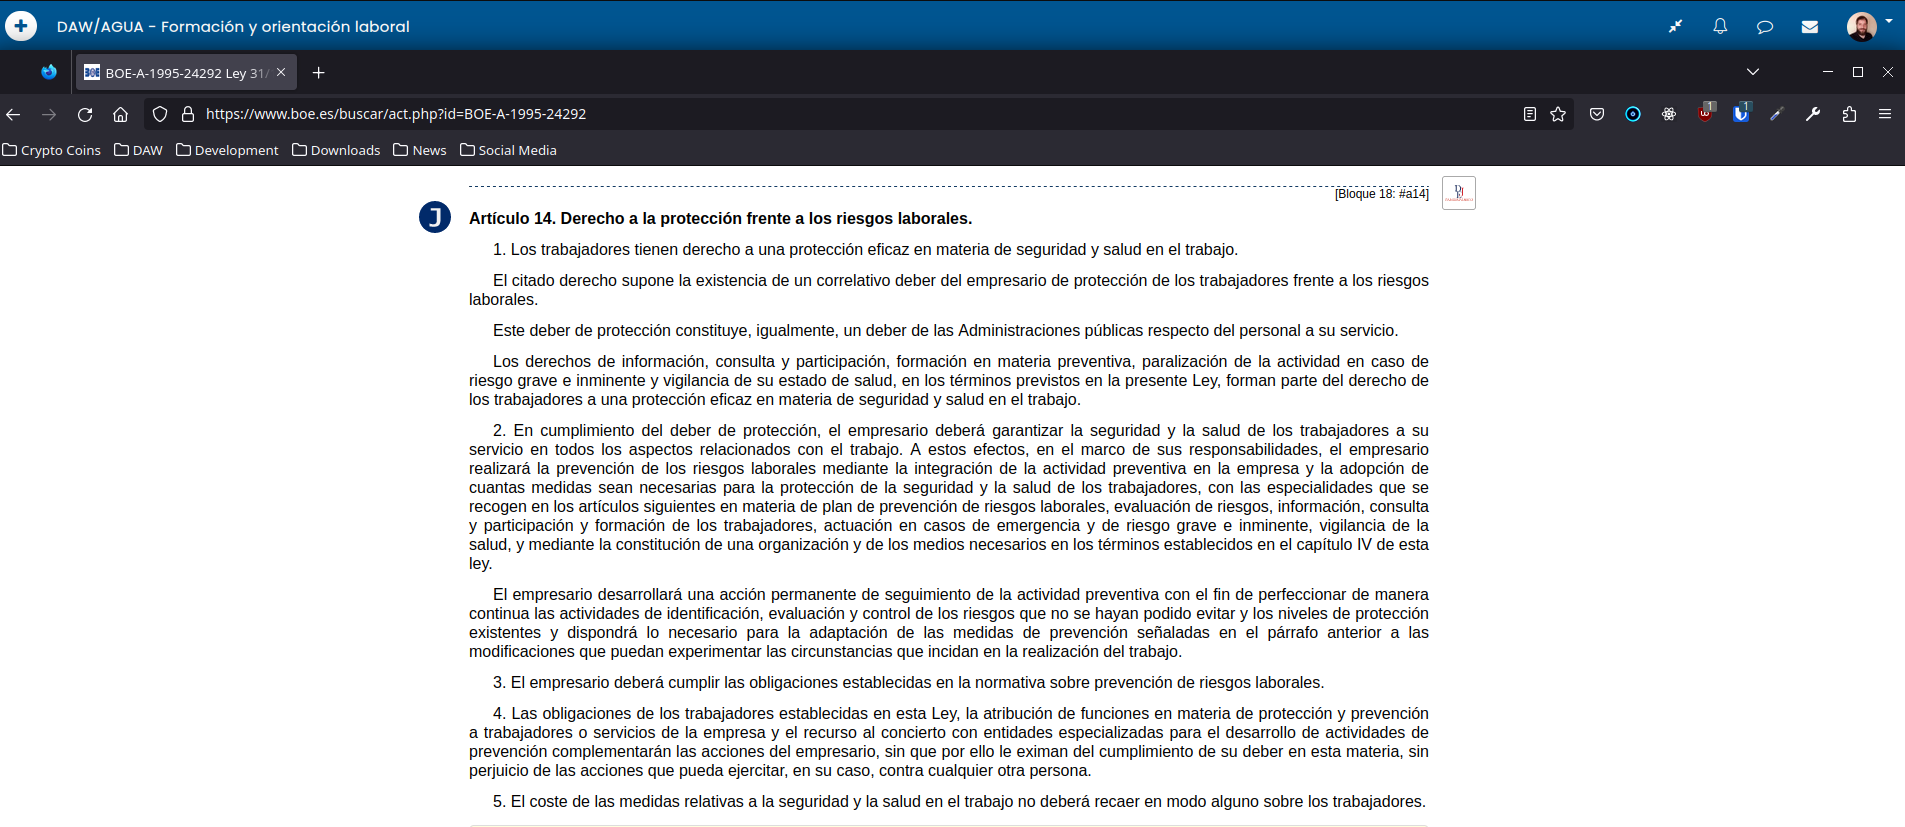
\includegraphics[scale=0.30]{derecho-trabajador.png}
        \caption{Articulo 14 de la LPRL}
    \end{figure}

    Este es un derecho que en \textbf{muchos casos no se cumple}, especialmente en el \textbf{sector de la construcción}, donde se obliga a los trabajadores a trabajar con condiciones climáticas a veces extremas, hablando en términos de calor, especialmente en verano, a pesar de que es evidente que hay un riesgo grave de sufrir un golpe de calor.

    Se suele implementar una jornada intensiva, pero está acaba a las 3 o 4 de la tarde, lo que quiere decir que a las horas de más calor del día, los trabajadores siguen en su puesto, trabajando.


    \item Para el \textbf{deber} del trabajador hemos elegido el \textbf{punto 5º} del \textbf{art 29} de la LPRL. Que dice los siguiente:

    ``\textit{Informar de inmediato a su superior jerárquico directo, y a los trabajadores designados para realizar actividades de protección y de prevención o, en su caso, al servicio de prevención, acerca de cualquier situación que, a su juicio, entrañe, por motivos razonables, un riesgo para la seguridad y la salud de los trabajadores}''

    En la siguiente captura podemos ver dicho artículo.

    \begin{figure}[H]
        \centering
        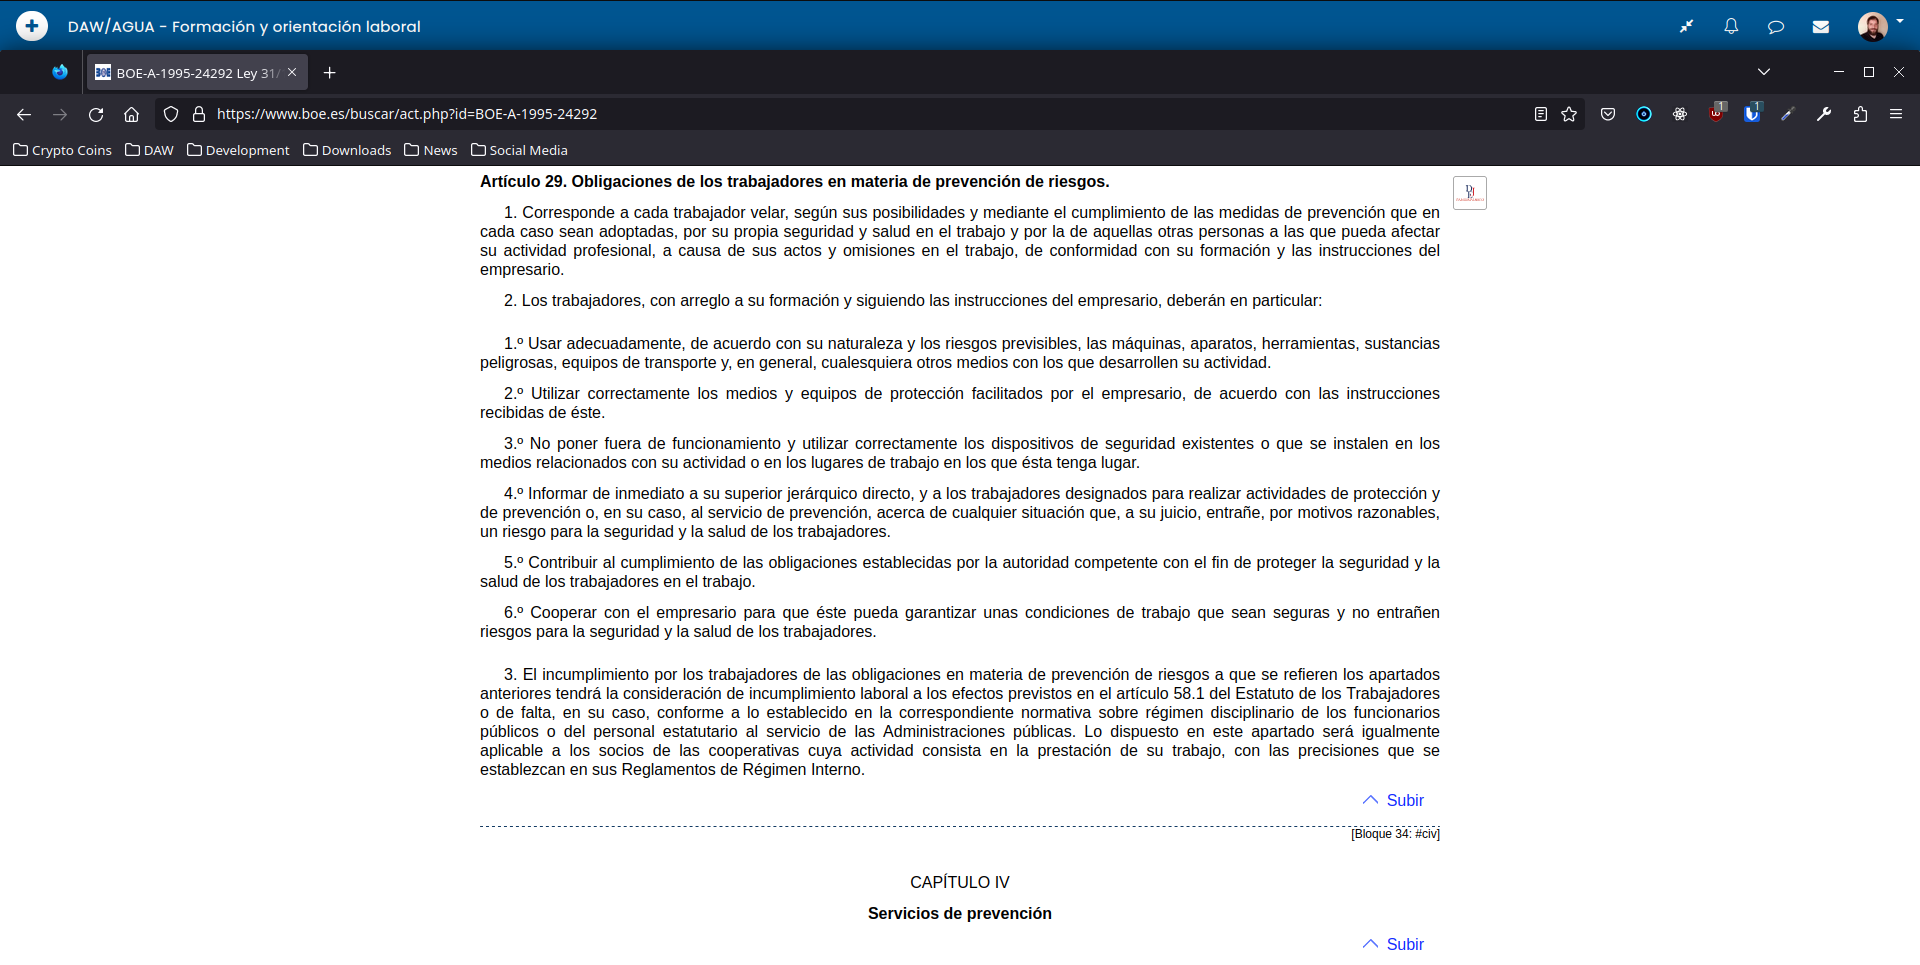
\includegraphics[scale=0.30]{deberes-trabajador.png}
        \caption{Artículo 29 de la LPRL}
    \end{figure}

    He escogido este artículo porque considero que puede ser uno de los más \textbf{conflictivos} de cumplir. Por ejemplo, estando en el puesto de trabajo, puede ser que haya compañeros que cumplan las medidas de seguridad. El simple hecho de informar a un superior es algo fácil de hacer, pero esto puede \textbf{generar conflictos} con los compañeros involucrados. Por lo tanto, creo que puede ser problemático, porque aunque está claro que se debe informar a un superior, entran otras variables en juego, como cuanto es de peligroso el incumplimiento, la relación que se tenga con el/los trabajadores involucrados, etc...
\end{enumerate}

\subsection{Actividad 2}

\subsubsection{Enunciado}
Explica las diferentes modalidades de llevar a cabo la organización de la prevención en la empresa a través de uno o varios ejemplos real/es o ficticio/s. No se trata de exponer las características de cada modalidad y poner un ejemplo sino más bien poniendo un ejemplo definir las características de la modalidad.

\subsubsection{Solución}
En este ejercicio vamos a poner un ejemplo de un situación ficticia y a determinar, explicando sus características, que modalidad organización de los servicios preventivos representan.

\begin{itemize}
    \item ``\textit{En el Bar Manolo, donde además de propietario hay 5 trabajadores, éste ha establecido una política de prevención de riesgos laborales básica, que ha formalizado en un documento que entrega a cada trabajador en el momento de firmar el contrato}. Además, tiene contratada una mutua donde se le realiza un chequeo anual a cada trabajador''.


    En esta situación, estaríamos ante la \textbf{modalidad} donde \textbf{el empresario asumirá personalmente la acción preventiva}. Esto puede ser así ya que cumple todas las características:

    \begin{enumerate}
        \item En primer lugar, estamos ante una empresa de menos de 15 trabajadores, y que tampoco desarrolla ninguna de las actividades peligrosas recogidas en el Anexo I del Reglamento de Servicios de prevención.
        \item Además, es propietario trabaja también en el bar y aunque no se menciona, tiene realizado un curso de prevención de riesgos laborales de 30h, por lo que también cumpliría el punto 2.
        \item Además, la vigilancia de la salud esta a cargo de una mutua, que ha contratado el propietario.
    \end{enumerate}

    \item \textit{``En el Supermercado SuperOFerta, la propietaria, Loli, que es su encargada, ha designado a una de sus empleadas, la que tiene mayor antigüedad y varios cursos de prevención de riesgos laborales, como la responsable de elaborar un plan de riesgos y encargarse de su cumplimiento. En el supermercado hay 10 trabajadores/as, pero la propietaria no suele estar en el local.}

    En este caso, la modalidad sería la de \textbf{designar un trabajador para llevarlo a cabo todo}. Se engloba dentro de esta modalidad por que, aunque podría englobarse en la del punto anterior, la empresaria \textbf{no desarrolla su actividad} en el supermercado, por lo que le resultaría imposible comprobar el cumplimiento del  plan de riesgos. En su lugar, ha \textbf{delegado esta responsabilidad} en su encargada, la que puede encargarse del cumplimiento de este plan.

    \item \textit{``En la empresa multinacional TodoSoftware, con más de 700 empleados, la junta directiva ha decidido instaurar el departamento de Prevención de Riesgos Laborales, ya que quieren llevar el control de este servicio, que se encargar de elaborar un plan adecuado de prevención así como de que éste se cumpla. Para ello, han realizado la contratación de 20 profesionales formados en la prevención de riesgos laborales para dicho departamento."}

    Esta modalidad sería la de \textbf{constituir un servicio de prevención propio}. Se ha optado por esta modalidad porque la empresa cumple con 2 de las tres condiciones que establece la normativa, a saber:

    \begin{enumerate}
        \item La empresa tiene más de 500 trabajadores, por lo que es obligatorio la creación de un servicio de prevención de riesgos laborales.
        \item Este segundo punto no lo cumple, ya que la empresa no desarrolla una actividad peligrosa, aunque si tiene más de de 250 trabajadores.
        \item Este punto también se cumple, ya que la empresa ha decidido crear ellos el servicio para llevar más control sobre éste, en vez de contratar a una empresa externa. Aún así, la empresa ya estaba obligada, ya que cumple el primer punto.
    \end{enumerate}

    \item \textit{``En la siderúrgica MetalChof, con 120 empleados, han decidido contratar una empresa externa que ofrezca los servicios de prevención de riesgos laborales, ya que está es una actividad de alto riesgos y tiene que haber profesionales bien formados en la prevención y económicamente, supone menos gasto contratar una empresa externa que montar su propio servicio, por lo que se ha contratado a la empresa CarbonizadosNO especializada en la prevención de riesgos laborales en el sector del metal.}''

    En este caso estaríamos ante la modalidad de \textbf{recurrir a servicios externos}, ya que se cumplen 2 de las tres características que definen a esta modalidad, que son:
    \begin{enumerate}
        \item La designación de uno o varios trabajadores no cubriría las necesidades de prevención de la empresa, ya que es un trabajo peligroso y la prevención de riesgos es más compleja que en otro tipo de trabajo, por lo que hace falta gente con alta formación para elaborar y controlar la prevención de riesgos laborales.

        \item También se cumple este punto, ya que la empresa no ha optado por por crear su propio servicio de prevención, resultando más barato la contratación de una empresa externa.

        \item Este punto no se cumple, básicamente porque es inviable que las funciones preventivas las desarrolle el empresario o los trabajadores, por lo que no se haría como complemento a esta circunstancia.
    \end{enumerate}
\end{itemize}


\subsection{Actividad 3}
\subsubsection{Enunciado}
De los órganos de representación en materia de Seguridad y Salud Laboral en la empresa:

\begin{enumerate}[label=\alph*.]
    \item Indica y explica brevemente los órganos de representación de la persona trabajadora en materia de Seguridad y Salud Laboral.
    \item Explica brevemente y de forma general sus funciones.
    \item ¿Qué es lo determinante para establecer el número de representantes (en materia de seguridad y salud) que debe tener una empresa?
    \item Una vez leídas las garantías de los  representantes de los trabajadores, justifica la necesidad de las mismas.
    \item Captura una garantía, la que sea de tu interés o te llame más la atención y justifica la elección.
\end{enumerate}

\subsubsection{Solución}
En esta actividad vamos a hablar sobre los \textbf{órganos de representación} de los trabajadores en materia de prevención en una empresa.

\begin{enumerate}[label=\alph*.]
    \item Los \textbf{principales órganos de representación} de los trabajadores son:
    \begin{itemize}
        \item \textbf{Delegados y Delegadas de Prevención}: son los representantes de los trabajadores en temas de prevención a los que además se les atribuye una función de vigilancia y control sobre el cumplimiento de la normativa.
        \item \textbf{Comité de Seguridad y Salud}: órgano de representación donde además de los trabajadores, está representada la empresa, teniendo dicha representación el mismo número para ambas partes.
    \end{itemize}

    \item Las principales funciones de ambos órganos de representación son las siguientes:
    \begin{itemize}
        \item \textbf{Delegados/as de Prevención}: como hemos dicho, representan a los trabajadores en materia de prevención en la empresa. Cualquier empresa con más de 6 trabajadores debe tener delegados de prevención, cuyo número variará en función del número de trabajadores. Sus principales \textbf{funciones} son:
        \begin{itemize}
            \item Colaborar con la dirección de la empresa en la mejora de la acción preventiva.
            \item Promover y fomentar la cooperación de los trabajadores en la ejecución de la normativa sobre prevención de riesgos laborales.
            \item Ser consultados por el empresario, con carácter previo a su ejecución, de las medidas y decisiones que se vayan a tomar en materia de prevención laboral.
            \item Ejercer una labor de vigilancia y control sobre el cumplimiento de la normativa en materia de prevención.
        \end{itemize}

        \item \textbf{Comité de Seguridad y Salud}: como ya hemos dicho, éste es un órgano donde tiene representación tanto los trabajadores como la empresa, siendo esta representación paritaria. Cualquier empresa con más de 50 trabajadores tiene que constituir un comité de salud y seguridad. Sus principales funciones son:
        \begin{itemize}
            \item Participar en todo lo referente a la elaboración, puesta en práctica y evaluación de los planes de prevención.
            \item Promover iniciativas sobre los métodos y procedimientos para hacer la prevención.
            \item Realizar las visitas oportunas para conocer la situación de la empresa en materia de seguridad y salud laboral.
            \item Tener acceso a la información necesaria para el correcto desarrollo de su actividad.
            \item Estar informado de las actividades del servicio de prevención, si hubiera uno.
            \item Conocer e informar de la memoria y programación anual de los servicios de prevención.
        \end{itemize}
    \end{itemize}

    \item Lo terminante para establecer el número de representantes es el \textbf{número de trabajadores} que tenga la empresa. Esto determinará el \textbf{número de delegados de prevención} y por extensión, el número de representantes de cada parte en el \textbf{comité de salud y seguridad}.

    \item Las \textbf{garantías de los representantes de los trabajadores} son muy necesarias, ya que facilitan el desempeño de su actividad, como el hecho de \textbf{no poder ser sancionado} o \textbf{despedidos} por el desempeño de sus funciones durante su mandaro, así como garantizan que siempre va a haber representantes de los trabajadores en al empresa, por ejemplo, teniendo preferencia a conservar el puestos en caso de un expediente regulador de empleo. Además, garantizan que la voz de los trabajadores se escuche, en materia de prevención.

    En conclusión, estas garantías son muy necesarias para el desarrollo de la actividad de los representantes de los trabajadores en materia de prevención.

    \item Las garantías aplicadas a los delegados de prevención de riesgos laborales son las establecidas en al \textbf{Art. 68} de \textbf{Estatuto de los Trabajadores}, referentes a los representantes de los trabajadores. En concreto, hemos elegido  el \textbf{apartado C}, como podemos ver en la siguiente captura.

    \begin{figure}[H]
        \centering
        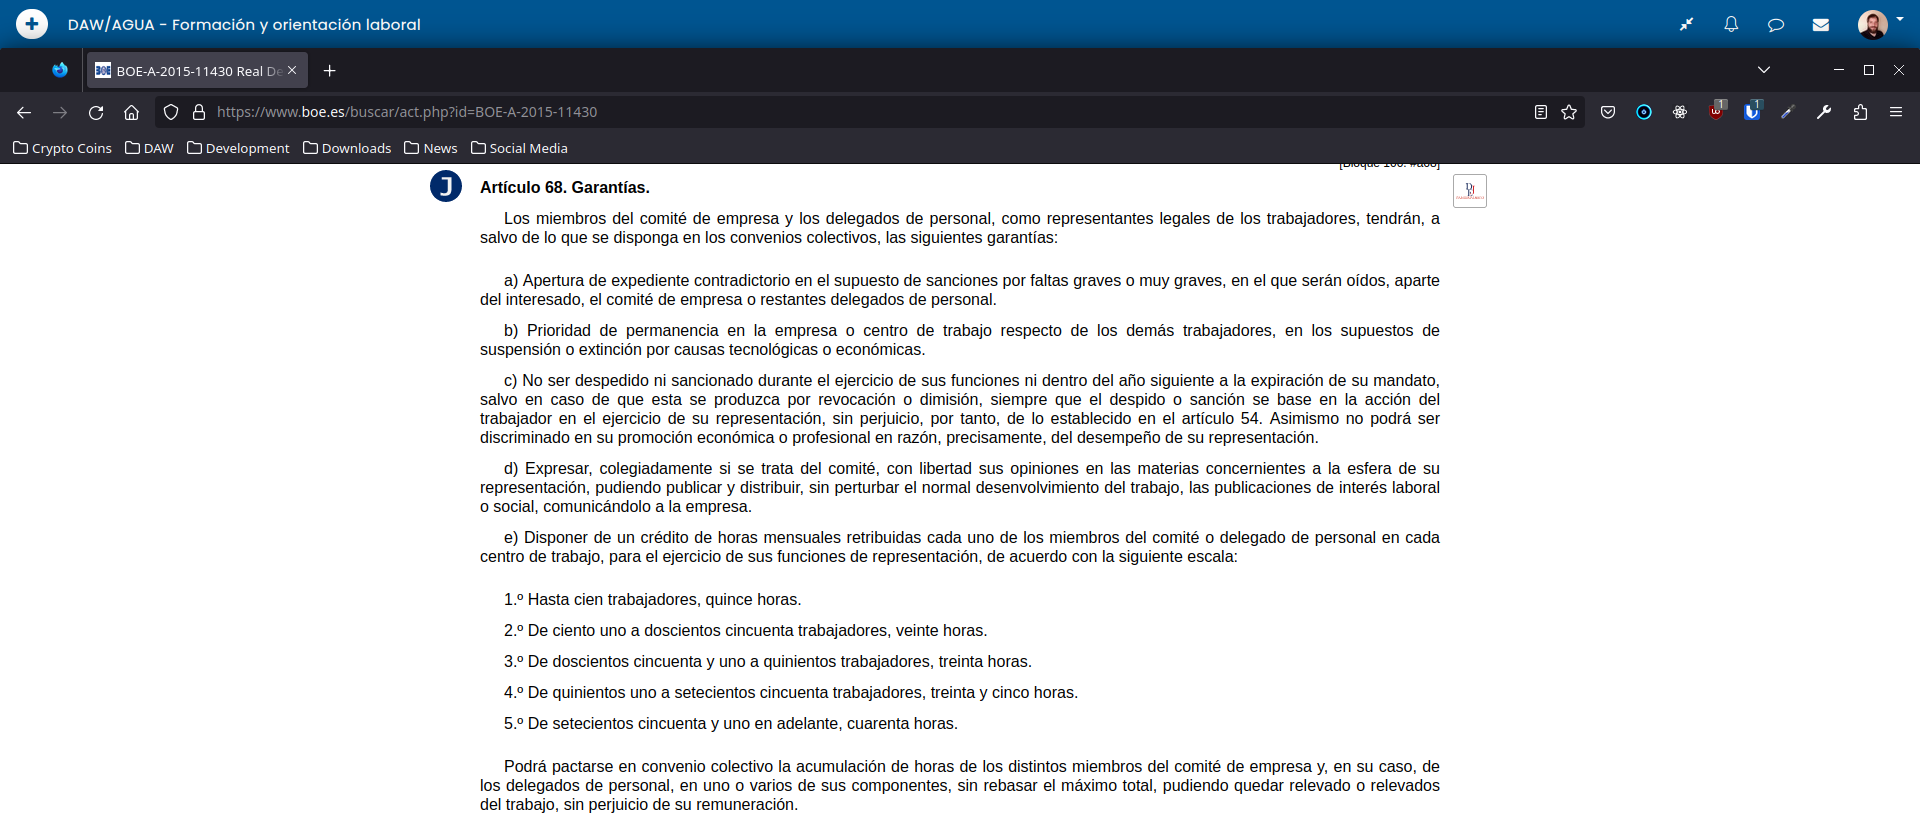
\includegraphics[scale=0.30]{garantias-delegados.png}
        \caption{Artículo 68 del Estatuto de los Trabajadores}
    \end{figure}

    En concreto el texto de este apartado dice:

    ``\textit{No ser despedido ni sancionado durante el ejercicio de sus funciones ni dentro del año siguiente a la expiración de su mandato, salvo en caso de que esta se produzca por revocación o dimisión, siempre que el despido o sanción se base en la acción del trabajador en el ejercicio de su representación, sin perjuicio, por tanto, de lo establecido en el artículo 54. Asimismo no podrá ser discriminado en su promoción económica o profesional en razón, precisamente, del desempeño de su representación}'' \cite{et01}

    Me parece \textbf{una garantía muy interesante y vital} para el desarrollo de la función de los delgados, ya que \textbf{evita} que se pueda \textbf{coaccionar} a los delegados para que tomen unas u otras decisiones con amenazas de sanción o despido por parte de la empresa.
\end{enumerate}

\subsection{Actividad 4}

\subsubsection{Enunciado}
De la evaluación de riesgos explica:
\begin{enumerate}
    \item Variables que se trabajan para catalogar o valorar los riesgos. Explica cada una de ellas.
    \item Significado de un riesgo calificado como ``tolerable''.
    \item Expón las medidas propuestas para el control de un riesgo calificado de ``intolerable''.
\end{enumerate}

\subsubsection{Solución}
En este punto, vamos a analizar un poco la evaluación de riesgos laborales.

\begin{enumerate}
    \item Las \textbf{principales variables} que se tienen en cuenta a la hora de catalogar un riesgos laboral son:
    \begin{itemize}
        \item \textbf{Magnitud}: esta variable se encarga de valorar la severidad del daño que puede causar ese riesgo, pudiendo ser esta \textbf{ligeramente dañino}, \textbf{dañino} o \textbf{muy dañino}.

        \item \textbf{Probabilidad de que Ocurra}: esta variable se encarga de medir la probabilidad de que ocurra un riesgo, teniendo en cuenta también la cantidad de trabajadores que se puedan ver afectados. La probabilidad puede ser \textbf{baja}, \textbf{media} o \textbf{alta}.


    \end{itemize}

     Uniendo estas dos variable, podemos realizar una clasificación de los riesgos laborales en \textbf{riesgo trivial}, \textbf{riesgo moderado}, \textbf{riesgo importante} y \textbf{riesgo intolerable}.

    \item Un \textbf{riesgo tolerable} es aquel con una magnitud (ligeramente dañino), es decir, que no provoca daños importantes, y con un probabilidad de que ocurra \textbf{baja} o \textbf{media}.

    Ante este tipo de riesgos, no se necesita una mejora de la acción preventiva, aunque se deben considerar mejoras que  no supongan una carga económica importante. Además, habrá que realizar comprobaciones periódicas para segurar que las medidas preventivas siguen siendo eficaces.

    \item Un \textbf{riesgo intolerable} es aquel con una magnitud (muy dañino), es decir, que puede provocar daños considerables, o incluso la muerte, en los trabajadores, y una probabilidad de se suceda \textbf{muy alta}.

    La \textbf{principal medida} de prevención de este tipo de riesgo es el \textbf{cese total de la actividad} de los \textbf{trabajadores expuestos} a él, la cual no se retomará mientras el riesgo subsista. Si no es posible reducir el riesgo, debe prohibirse la realización de este trabajo.
\end{enumerate}

\subsection{Actividad 5}
\subsubsection{Enunciado}
Contesta a las siguientes cuestiones:

\begin{enumerate}[label=\alph*.]
    \item Cita los instrumentos esenciales de gestión del plan de prevención.
    \item Justifica de forma clara y precisa las fases de la evaluación de riesgos.
    \item Ordena según el artículo 15 de la LPRL los siguientes principios que aparecen desordenados indicando al lado la numeración correcta en el orden que corresponde.
    \begin{itemize}
        \item Evaluar los riesgos que no se puedan evitar.  Nº
        \item Adaptar el trabajo a la persona. Nº
        \item Tener en cuenta la evolución de la técnica. Nº
        \item Planificar la prevención. Nº
        \item Sustituir lo peligroso. Nº
        \item Dar las debidas instrucciones a los trabajadores. Nº
        \item Adoptar medidas que antepongan la protección colectiva a la individual. Nº
        \item Evitar los riesgos. Nº
        \item Combatir los riesgos en su origen. Nº
    \end{itemize}
\end{enumerate}

\subsubsection{Solución}
En esta actividad vamos a seguir respondiendo cuestiones sobre la evaluación y prevención de riesgos laborales.

\begin{enumerate}[label=\alph*.]
    \item Las \textbf{principales herramientas} de gestión del plan de prevención son:
    \begin{itemize}
        \item \textbf{Evaluación de Riesgos Laborales}
        \item \textbf{Planificación de las Actividades Preventivas}
    \end{itemize}

    \item Las fases de evaluación de riesgos son las siguientes:
    \begin{enumerate}
        \item \textbf{Analizar el Riesgo}: en esta fase de analiza el riesgo, utilizando para ello un cuestionario o guía que nos permita describir e identificar el riesgo. Existen diferentes métodos de evaluación de riesgos como el \textbf{método EWA} o el \textbf{método PYMES}.

        Esta fase es importante dentro del proceso de evaluación, ya que para poder actuar sobre un riesgo laboral lo primero es poder tener identificado ese riesgo, sino, difícilmente se van a pode tomar acciones preventivas.

        \item \textbf{Estimar el Riesgo}: en este fase se estima la \textbf{magnitud} del riesgo, es decir, la \textbf{severidad del daño que este puede causar}, y la \textbf{probabilidad de que ocurra}, teniendo ademas en cuenta el número de personas que se pueden ver afectadas.

        Es importante conocer el alcance que tiene cada riesgo, ya que dependiendo de este, deberán tomarse medidas más o menos severas.

        \item \textbf{Valoración}: en esta última etapa del proceso se valora el riesgo, teniendo ya descrita su magnitud y la posibilidad de que suceda, hay que usar estas dos variables para determinar el tipo de riesgo ante el que estamos, tomando medidas más ligeras o más severas dependiendo de ésto.

        Esta última fase es determinante, ya que aquí se determina con precisión, en función de su magnitud y probabilidad de que suceda, el tipo de riesgo que estamos tratando, que será el punto de partida para elaborar la planificación de la prevención sobre ese tipo de riesgo concreto.
    \end{enumerate}

    \item Según la LPRL \cite{lprl01}, la ordenación quedaría de la siguiente forma:

        \begin{itemize}
        \item Evaluar los riesgos que no se puedan evitar.  \textbf{Nº 2}
        \item Adaptar el trabajo a la persona. \textbf{Nº 4}
        \item Tener en cuenta la evolución de la técnica. \textbf{Nº 5}
        \item Planificar la prevención. \textbf{Nº 7}
        \item Sustituir lo peligroso. \textbf{Nº 6}
        \item Dar las debidas instrucciones a los trabajadores. \textbf{Nº 9}
        \item Adoptar medidas que antepongan la protección colectiva a la individual. \textbf{Nº 8}
        \item Evitar los riesgos. \textbf{Nº 1}
        \item Combatir los riesgos en su origen. \textbf{Nº 3}
    \end{itemize}
\end{enumerate}

\subsection{Actividad 6}

\subsubsection{Enunciado}
Analiza el artículo 20 de la LPRL y haz una valoración de su contenido.

\subsubsection{Solución}
El \textbf{Artículo 20 de la LPRL} trata sobre las \textbf{medidas de emergencia}. En aspecto, el responsable de organizar esas medias es \textbf{el empresario}, debiendo hacerse cargo de nombrar a las personas que sean necesarias como responsables de poner en práctica estas medidas, teniendo este personal que tener la formación necesaria en prevención de riesgos laborales.

Además, el empresario deberá contratar los \textbf{servicios externos} necesarios para el correcto funcionamiento y cumplimiento de las medidas de emergencia, especialmente en materia de auxilios, asistencia médica de urgencia, salvamento o lucha contra incendios.

Como vemos, este articulo deja claro que \textbf{toda la responsabilidad} de la planificación de las medidas de emergencia es del \textbf{empresario}, por lo que en caso de incumplimiento puede haber sanciones cuya gravedad dependerá también de como de grave sea la negligencia por parte de este, aunque dependiendo.

\subsection{Actividad 7}

\subsubsection{Enunciado}
\begin{enumerate}[label=\alph*.]
    \item ¿Juega la inspección de trabajo algún papel fundamental respecto a la prevención de riesgos?
    \item Si una persona trabajadora incumpliera de manera continua y sistemática sus obligaciones y deberes en materia de prevención.
    \begin{itemize}
        \item ¿Cuáles son sus responsabilidades a nivel laboral?. Justifica la respuesta.
        \item Indica a quien/es le corresponde sancionar dichos incumplimientos.
        \item Expón las consecuencias que para el trabajador se derivan por dicho incumplimiento.
    \end{itemize}

    \item Cita tipos de responsabilidad :
    \begin{itemize}
        \item Para la persona trabajadora.
        \item Para la empresa.
    \end{itemize}
\end{enumerate}

\subsubsection{Solución}
Es esta última actividad, vamos a trabajar un poco las \textbf{responsabilidades y sanciones} en la prevención de riesgos laborales.

\begin{enumerate}
    \item La \textbf{Inspección de Trabajo}, juega un papel fundamentar en la prevención de riesgos laborales. Según el \textbf{Artículo 9 de la LPRL}, corresponde a la Inspección de Trabajo, junto a la Seguridad Social, la \textbf{vigilancia y el control} de la normativa de sobre prevención de riesgos laborales, siendo los encargados de tramitar los expedientes de infracción y elevar a la autoridad  laboral las propuestas de sanción.

    \item En el caso de que una persona incumpliera de manera continua la legislación:

    \begin{enumerate}
        \item En caso de un \textbf{trabajador}, se puede enfrentar a sanciones dentro de la empresa que dependerá del tipo de infracción, pudiendo ser estas desde \textbf{leves} a \textbf{muy graves}.
        \item La \textbf{responsable de sancionar} a los trabajadores que incumplen la normativa de prevención de riesgos laborales es la empresa.
        \item Las \textbf{consecuencias} dependerán de la \textbf{gravedad de la infracción}, pudiendo ir desde una simple amonestación en los casos de infracciones leves hasta el despido, en las infracciones muy graves. El tipo de sanciones y de infracciones estarán estipuladas en el \textbf{convenio colectivo}.
    \end{enumerate}

    \item Los tipos de responsabilidad que puede tener cada parte en una relación laboral son:
    \begin{itemize}
        \item \textbf{Trabajadores}: en este caso, los trabajadores pueden verse afectados por la \textbf{responsabilidad laboral}, no pudiendo tener responsabilidad administrativa ya que no lo recoge la Ley Sobre Infracciones y Orden Social.

        \item \textbf{Empresa}: los empresarios, por otro lado, pueden tener \textbf{responsabilidad administrativa}, \textbf{civil} y \textbf{penal}.
    \end{itemize}
\end{enumerate}


% Bibliography

\newpage
\bibliography{citas}
\bibliographystyle{unsrt}

\end{document}